\section{Discussion}

\label{sec:discussion}It is well known that the accretion processes
of black holes and the resultant energy deposition into the host galaxy
are necessary ingredients in the evolution of galaxies over cosmic
time. Although we do not fully understand the causal relationship
between the black hole and its host galaxy, our ability to constrain
the mechanisms responsible are derived principally from simulations
of the phenomena. Using the Illustris-2 simulation, we are able to
quantify the growth and evolution of supermassive black holes in a
cosmological simulation at the resolution of $\sim10^{5}\,{\rm M_{\odot}}$
over cosmic time.

In Figure \ref{fig:bhpop_hist2d}, we find that the accretion rate
of black holes with masses less than the median mass of $7.04\times10^{5}\,{\rm M}_{\odot}$
exhibit a range of accretion rates from $\sim10^{-16}$ to $\sim10^{-11}\,{\rm M_{\odot}}\, s^{-1}$.
Assuming these black holes have always been growing at these rates,
then on the average they must accrete for more than $3$ Hubble times
in order to achieve the median black hole mass today even though their
seed mass is $1.42\times10^{5}\,{\rm M_{\odot}}$. Hence, their current
accretion rates are too low to account for their masses at $z=0$.
Examining black holes with masses larger than the median, we find
a similar result. For example, a typical $10^{7}\,{\rm M}_{\odot}$
black hole is accreting at approximately $10^{-12}{\rm M}_{\odot}s^{-1}$
at $z=0$. At this rate, such a black hole could only yield a mass
of $\sim10^{5}{\rm M}_{\odot}$ over the simulation time. Additionally,
this trend holds for the black holes with current masses in excess
of $10^{9}\,{\rm M_{\odot}}$ which generally exhibit accretion rates
above $\dot{{\rm M}}\ge10^{-9}{\rm M}_{\odot}s^{-1}$. The same calculation
as above yields a mass of $\sim10^{8}{\rm M}_{\odot}$ over the simulation
time. This strongly suggests that the accretion rates for all black
holes in the Ilustris simulation were likely much larger in the past.
This is consistent with the notion that black hole accretion rates
are tied to the gas fraction in galaxies which is known to be larger
at higher redshift \citep{bauermeister2013theegnog}.

Examing the gas masses of the groups to which our sample of black
holes belongs (see Figure \ref{fig:mgroup_vs_mgas}), we find that
the groups with the largest masses contain both the largest gas masses
as well as the largest mass black holes. This is consistent with the
scenario in which the group dark matter halo grows hierarchically
creating an ever larger gravitational potential into which the cosmic
gas falls. This feeds the central black hole thereby allowing its
mass to increase in lockstep with the mass of the group halo. From
Figure \ref{fig:Mdot_vs_Mgas}, we see that the most massive black
holes live in the most gas poor halos (i.e., have the smallest gas
masses for their host halo masses) but, seemingly paradoxically, have
the highest accretion rates today.

Clearly then, a substantial portion of the gas in these groups must
be present in the center of the halo in order to feed the black hole
(assuming the black hole lives at the center of the halo). However,
this gas must have a temperature below the virial temperature of the
halo in order to aggregate in the center of the halo. This indicates
that the gas deposited into these halos likely comes from the cosmic
filaments rather than from smaller galaxies merging into the group
which would be shock heated as they fall into the halo. How, then,
can this relatively cold gas still be present in these groups when
the accretion rates are nearly four orders of magnitude greater than
those of black holes at the median mass of our sample and these black
holes have masses requiring timescales longer than the simulation
time to achieve even at their current accretion rates? One possibility
is that the gas has only recently fallen into the halo. However, it
is unlikely that $\sim10^{14}\,{\rm M_{\odot}}$ of gas suddenly appears
in a halo at $z\sim0$. Another possibility is that these black holes
have only recently become active, consuming the gas supply that has
been building over cosmic time, and providing their host galaxies
with a large energy feedback.

Conversely, the lowest mass black holes live in the most gas rich
halos yet exhibit the lowest accretion rates. This indicates that
the gas in these groups is likely diffuse and unable to coalesce onto
the central black hole. This may be due to the black holes in these
groups having undergone intense energy output at earlier times, heating
and pushing the gas toward the outer regions of the halo. Although
we do not have the temperature and density measurements to fully quantify
this, we note that this is consistent with our previous findings that
these low-mass black holes could not have grown to their current masses
in less than $\sim3$ Hubble times and must have been accreting at
a higher rate in the past. This appears to be a ``downsizing'' of
black hole accretion rates similar to the downsizing seen with the
cosmic specific star formation rate \citep{damen2009theevolution}.

This dichotomy in black hole accretion rates, discussed further in
\citet{sijacki2014theillustris}, seemingly implies the presence of
two black hole populations in the Illustris simulation. However, we
find that our sample of black holes reproduces the slope of the fundamental
plane from M03 to within a factor of $\sim2$. If there were indeed
two separate populations of black holes providing fundamentally different
mechanisms of energetic feedback to their host galaxies, their X-ray
luminosities would not be so closely tied to their mass accretion
rates as indicated by the tight correlation on the fundamental plane.

\begin{figure}
\begin{centering}
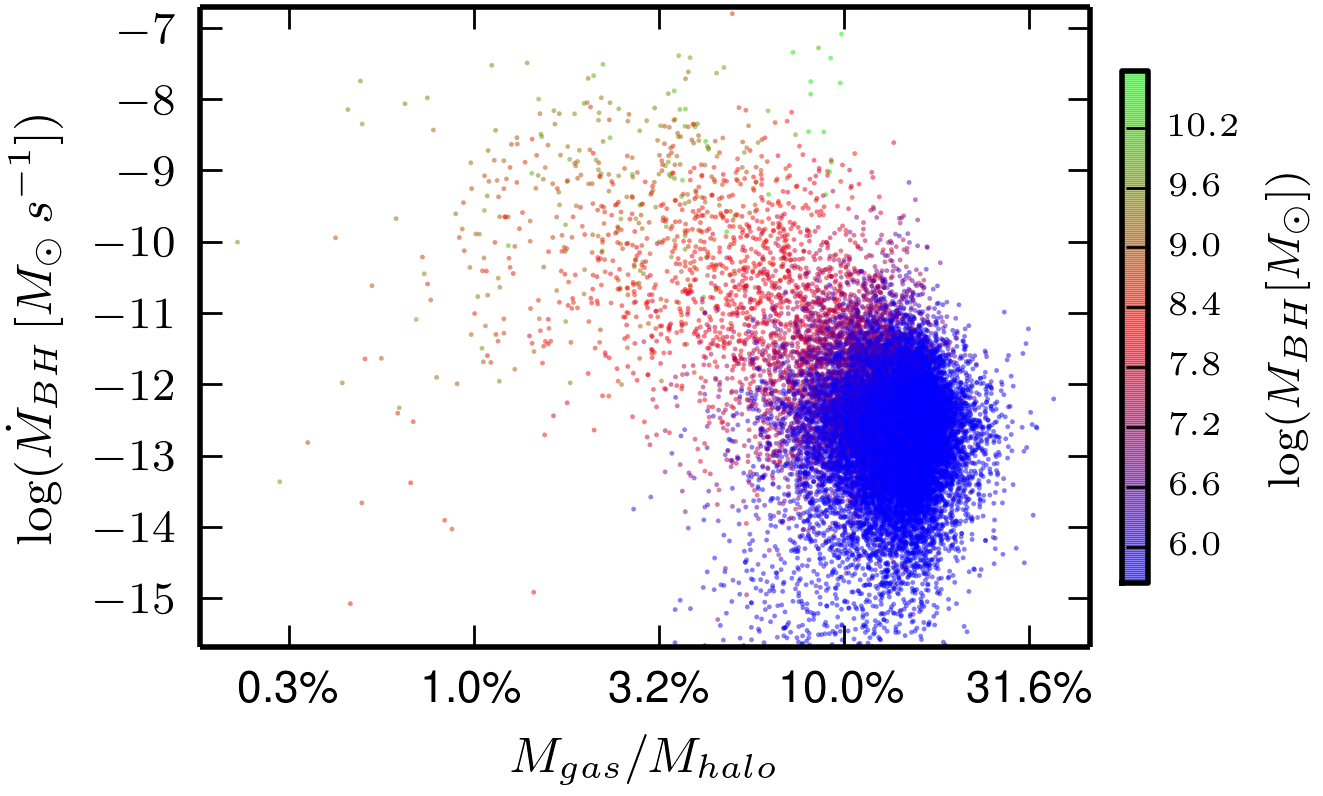
\includegraphics{Figures/Mdot_vs_GasFrac}
\par\end{centering}

\protect\caption{\textbf{\label{fig:Mdot_vs_Mgas}}Black hole accretion rate of as
a function of the fraction of gas in each group for our sample. Colors
correspond to black hole mass. All masses are in units of $\log\left(M_{\odot}\right)$
and the accretion rate is in units $\log\left(M_{\odot}yr^{-1}\right)$.}


\end{figure}
\begin{figure}
\centering{}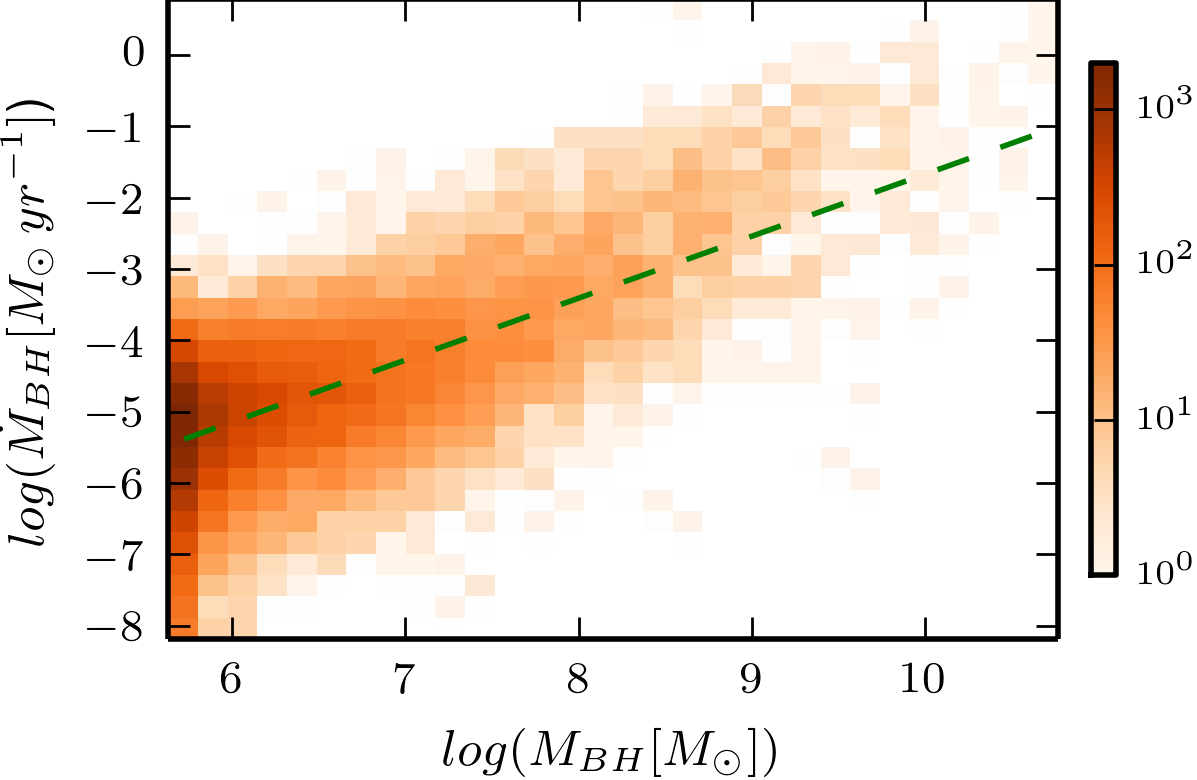
\includegraphics[clip]{Figures/Illustris2_bhpop_hist2d}\protect\caption{\label{fig:bhpop_hist2d}Black hole accretion rate as a function of
black hole mass for the Illustrist-2 simulation for our sample. Colors
correspond to a two-dimensional density of the same plot sampled in
log space.}
\end{figure}
\begin{figure}
\begin{centering}
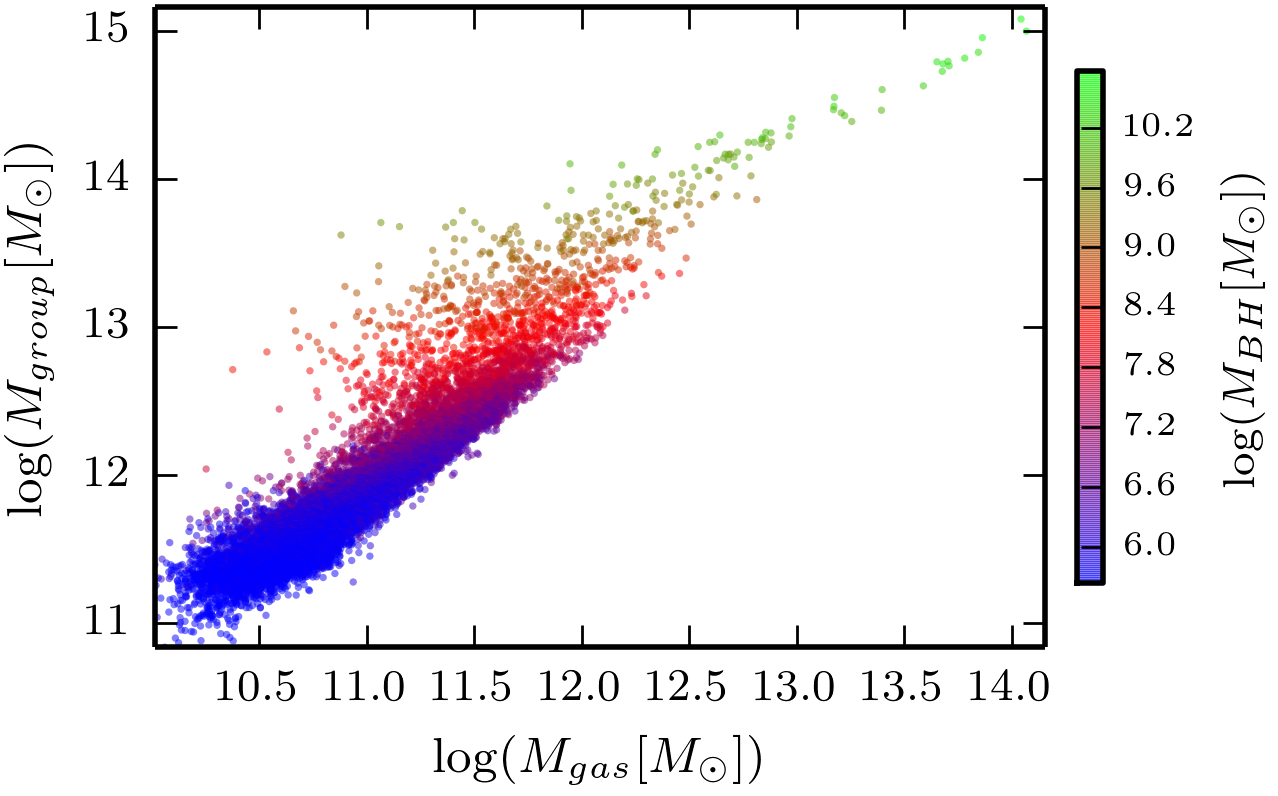
\includegraphics{Figures/Mgroup_vs_Mgas}
\par\end{centering}

\protect\caption{\label{fig:mgroup_vs_mgas}Group gas mass as a function of the group
mass for our sample of black holes from the Illustris simulation.
Colors correspond to the mass of the black holes. All units are in
${\rm M_{\odot}}$.}


\end{figure}
